\section{方法}

\begin{figure*}[t]
  \centering
  \vspace{0.5em}
  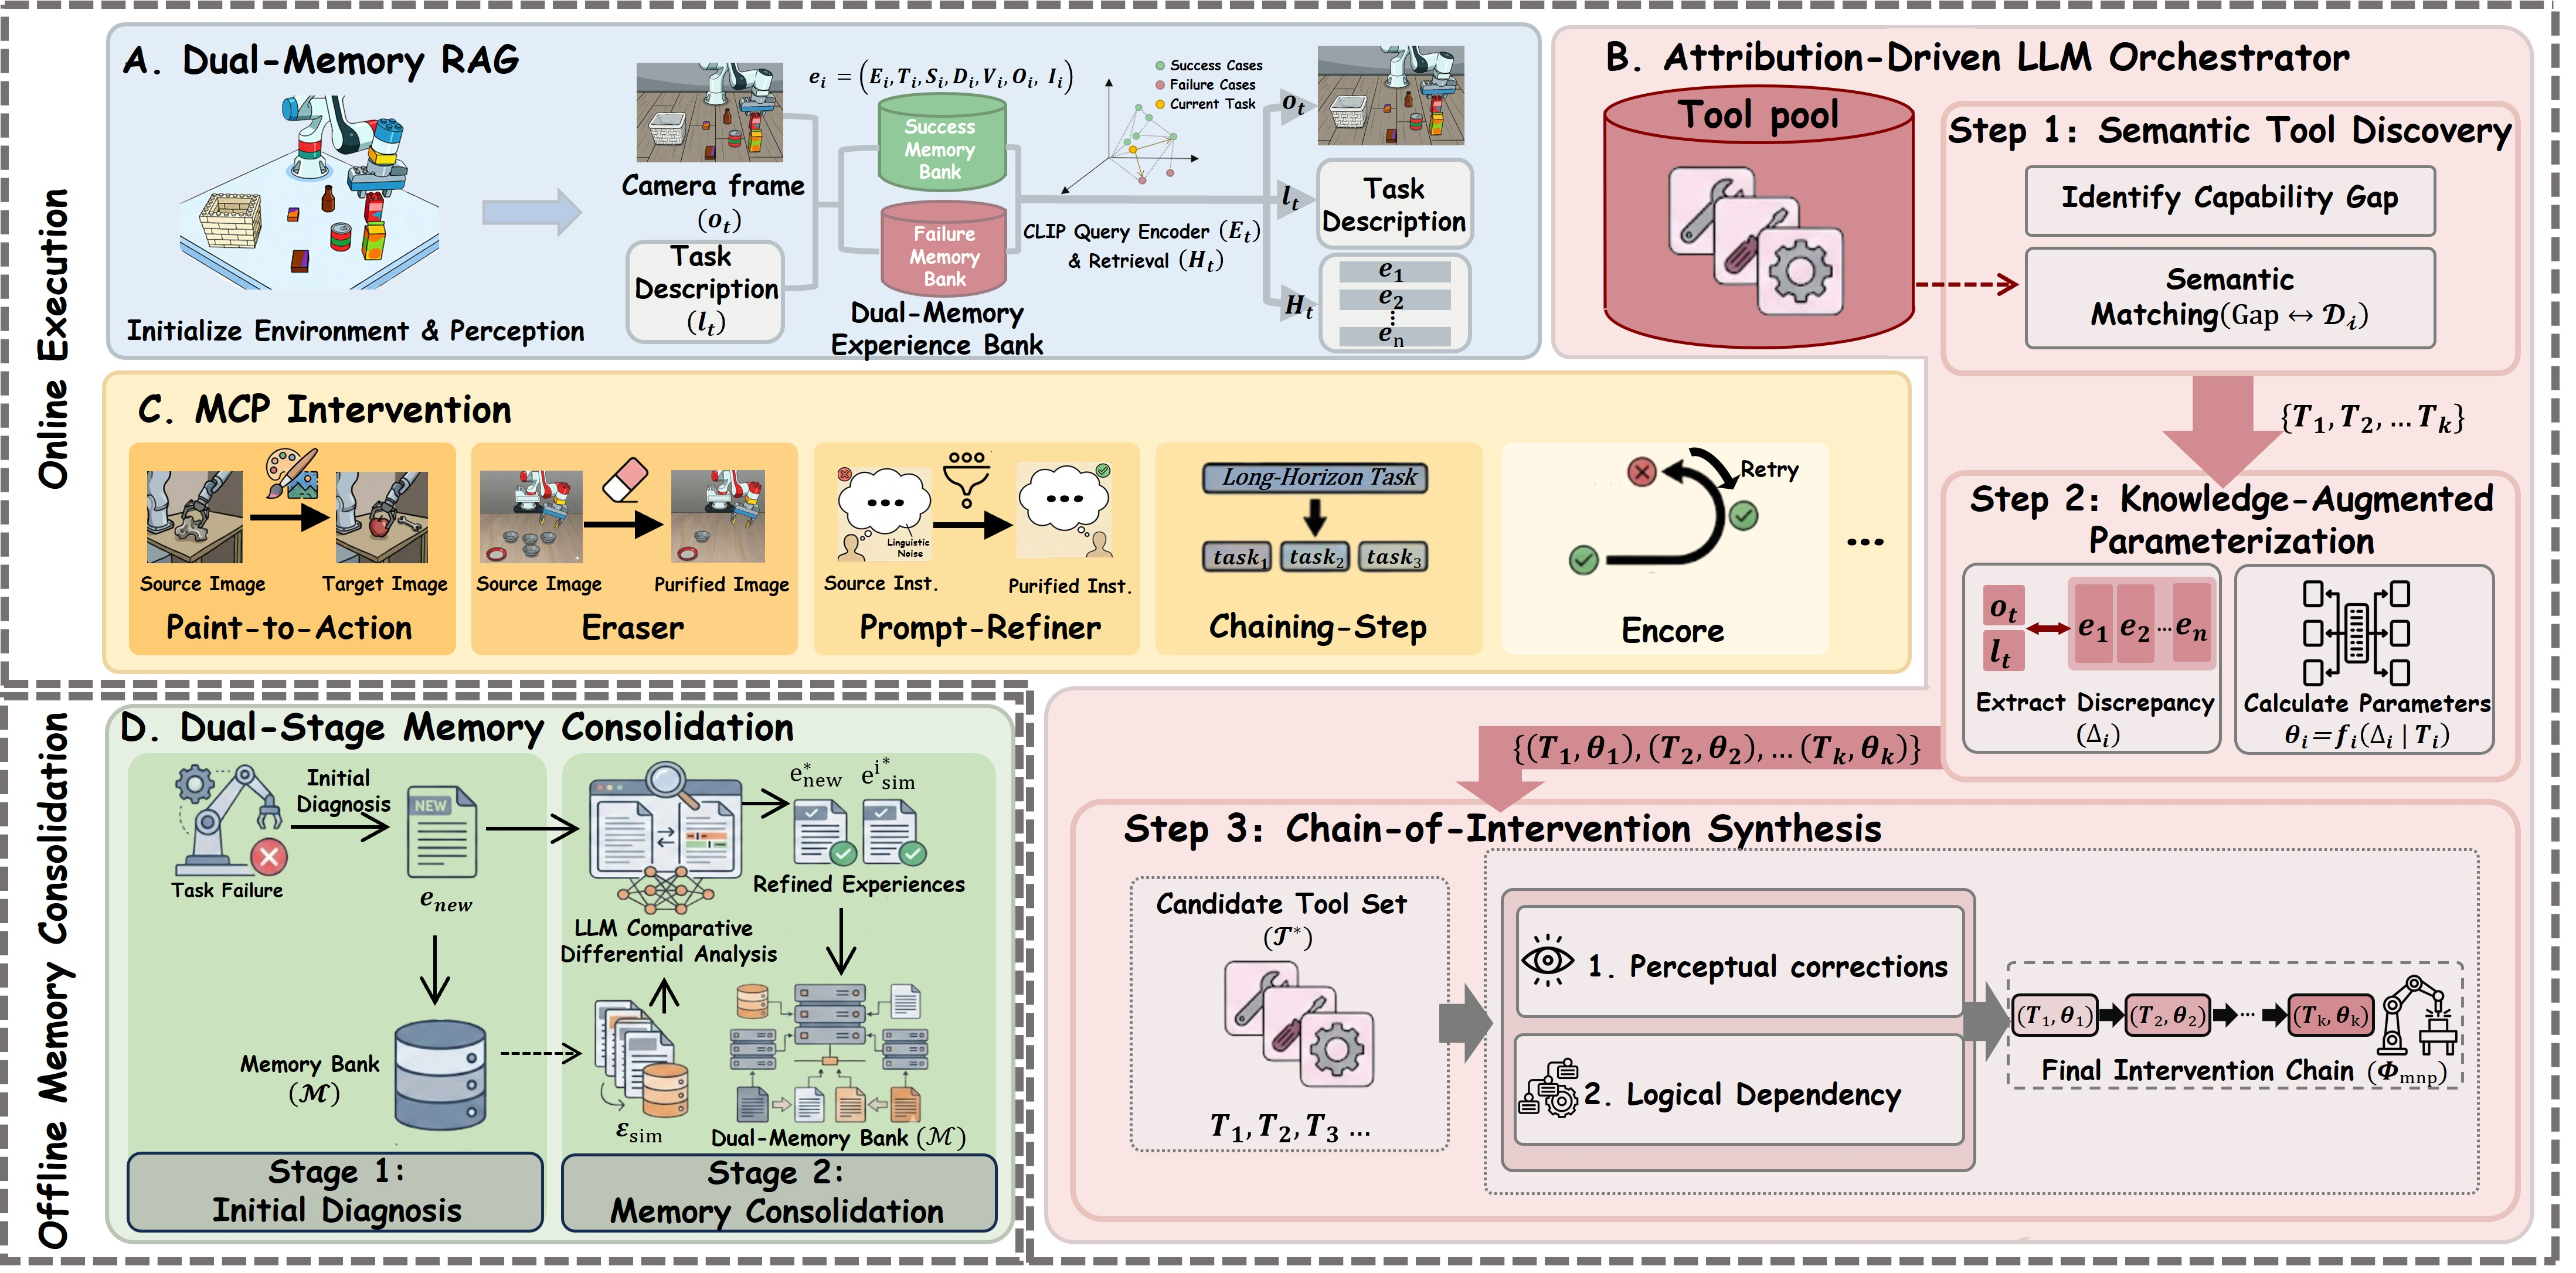
\includegraphics[width=0.85\linewidth]{figure/framework.jpg}
  \caption{\textbf{\sys\ 框架。}给定观测和指令，双记忆 RAG 从双记忆库检索相关经验。视觉--语言编排器选择 MCP 工具、估计参数 $\theta$，并合成由可扩展 MCP 工具执行的干预链。执行后，异步记忆巩固更新记忆库，闭合迭代改进回路。}
  \vspace{-1.5em}
  \label{framework}
\end{figure*}

本节介绍\textbf{\sys}框架。如图~\ref{framework} 所示，它由\textbf{在线执行工作流}和\textbf{离线记忆巩固工作流}组成。

\paragraph{在线执行工作流}
在线工作流通过三个模块实现鲁棒的任务级自适应：
\textbf{(1) 双记忆 RAG} 从双记忆库检索成功指导和失败警示；
\textbf{(2) 归因驱动的视觉--语言编排器}诊断障碍，并选择由归因指导的干预；
\textbf{(3) MCP 干预}通过调节感知和语言输入的可扩展工具执行这些干预。

\paragraph{离线记忆巩固工作流}
作为在线执行的补充，离线工作流进行\textbf{双阶段记忆巩固}。
它将新观测到的成功和失败轨迹提炼为结构化记忆并更新双记忆库，从而无需更新参数即可持续改进。

这两个工作流共同构成一个闭环自适应系统。
\vspace{-0.5em}
\[
\underbrace{
    \overbrace{\text{Obs.} \rightarrow \text{Retr.} \rightarrow \text{Dec.} \rightarrow \text{Orch.}}^{\substack{\text{任务级} \\ (\text{每项任务一次})}} \rightarrow \overset{\substack{\text{片段级} \\ (\text{每 } N \text{ 步})}}{\text{Exec.}}
}_{\text{在线}}
\rightarrow
\underbrace{\text{Consol.}}_{\text{离线}}
\]
下面详细介绍各模块。

\subsection{双记忆 RAG}
\label{dual memory}

图~\ref{framework}A 展示了一个检索增强的双记忆库，它使用先前的成功和失败经验为编排器的推理提供落地依据。
其\textbf{双重}设计将成功/失败经验分开以进行对比式归因，并通过双阶段巩固改进每个条目（第~\ref{Evolution} 节）。

下面介绍记忆库的构建过程及其检索机制。

\subsubsection{双记忆存储设计}

我们构建一个双分区记忆库：
\begin{equation}
\mathcal{M} = \mathcal{M}_{succ} \cup \mathcal{M}_{fail},
\end{equation}
其中，$\mathcal{M}_{succ}$ 将成功干预存为正向指导，$\mathcal{M}_{fail}$ 则将带有归因信号的失败尝试存为负面证据，以支持对可复用策略与应避免模式进行对比推理。

第~\ref{dual memory ablation} 节的消融表明，单分区记忆会导致规划不稳定或低效，而同时使用两个分区能够减少推理轮数及其方差。

每个经验条目 $e_i \in \mathcal{M}$ 都以半结构化模式存储：固定的核心模式辅以可扩展辅助字段：
\vspace{-0.5em}
\begin{equation}
e_i = \big(
\overbrace{E_i, T_i, S_i, D_i, V_i, O_i}^{\text{固定模式}},
\mathcal{I}_i
\big),
\end{equation}
\begin{itemize}
    \item $E_i$：任务实例的多模态嵌入；
    \item $T_i$：自然语言任务描述；
    \item $S_i \in \{0,1\}$：成功指示量；
    \item $D_i$：诊断标注（失败时非空）；
    \item $V_i$：执行视频的关键帧表征；
    \item $O_i$：表示为物体--属性对的结构化场景；
    \item $\mathcal{I}_i$：可扩展的结构化元数据包。
\end{itemize}

元数据包 $\mathcal{I}_i$ 存储 \texttt{key\_frame\_range}、\texttt{success\_max\_step} 和 \texttt{rollback} 等工具执行参数，同时允许随工具或推理信号演化而加入新字段。

\subsubsection{基于相似度的检索策略}

我们使用预训练 CLIP 编码器~\cite{CLIP} $E(\cdot, \cdot)$，将当前任务上下文（初始观测 $o_t$ 与指令 $l_t$）投影到联合嵌入空间。
检索形式化为：
\begin{equation}
\mathcal{H}_t = \text{Top-}k\Big(\text{Sim}\big(E(o_t, l_t), \{E_i \mid e_i \in \mathcal{M}\}\big)\Big),
\end{equation}
$\mathcal{H}_t$ 同时包含成功样例与失败先例，为归因驱动推理提供\textbf{正向指导}和\textbf{负向反事实}。

三元输入 $(\mathcal{H}_t, o_t, l_t)$ 为编排器诊断差异并安排适当干预工具的顺序提供了必要的落地依据。
\vspace{-0.5em}

\subsection{归因驱动的视觉--语言编排器}

如图~\ref{framework}B 所示，归因驱动的视觉--语言编排器是 \sys\ 的决策核心。
它由 Qwen3-VL-32B 驱动；这里把该多模态大语言模型（MLLM）用作视觉--语言模型，对观测、指令和检索到的视觉--语义记忆进行联合推理，以诊断执行失败并编排 MCP 干预。

\subsubsection{语义工具发现与意图对齐}

编排器通过度量当前状态 $o_t$ 与检索原型 $\mathcal{H}_t$ 之间的能力差距来确定干预。
给定语义工具描述 $\{\mathcal{D}_i\}_{i=1}^N$，它执行零样本匹配以选择候选工具集：
\begin{equation}
    \mathcal{T}_{1:k}= \text{Match}\big(\Delta_{g}, \{\mathcal{D}_i\}_{i=1}^N\big), \quad \Delta_{g} = \text{Gap}(o_t, \mathcal{H}_t),
\end{equation}
由此选择功能与诊断出的失败原因一致的工具。

\subsubsection{知识增强的参数化}
\label{Knowledge-Augmented Parameterization}

选定工具后，编排器从多模态上下文差异 $\Delta$ 推导执行参数 $\theta_i$：
\begin{equation}
 \theta_i = f(\Delta_i \mid T_i), \quad \Delta_i = \text{Gap}(o_t, l_t, \mathcal{H}_t\mid T_i),
\end{equation}
其中 $f$ 表示面向特定工具取值的映射函数。
具体而言，$\Delta$ 描述当前观测 $o_t$ 和指令 $l_t$ 相对于历史先验 $\mathcal{H}_t$ 在视觉、语义和时间维度上的偏差。
表~\ref{tab:parameterization_formal} 总结了如何把这些定量差异映射为各工具的具体执行参数 $\theta_i$。

\begin{table}[htbp]
\vspace{-1.5em}
\centering
\caption{面向特定工具的参数化映射。}
\label{tab:parameterization_formal}
\footnotesize
\renewcommand{\arraystretch}{1.25}
\begin{tabularx}{\columnwidth}{@{} l X l @{}}
\toprule
\textbf{工具} & \textbf{相对于 $\mathcal{H}_t$ 的差异 $\Delta$} & \textbf{$\theta_i$} \\
\midrule
Paint  & 与历史均值的特征距离。         & $C,\,M,\,A_{mask}$ \\
Eraser & 相对背景模型的新颖几何结构。   & $D,\,D_{masks}$ \\
Prompt & 与成功模式不匹配的指令。       & $\mathcal{S}_{origin}$ \\
Chain  & 子事件级对齐。                 & $(N_{e},N_{b})_k$ \\
Encore & 与历史失败轨迹的相似度。       & $[s_s,s_e],\,N_w$ \\
\bottomrule
\end{tabularx}
\vspace{3pt}
\begin{flushleft}
\scriptsize
\textbf{$C$}：颜色/纹理；\enspace
\textbf{$M$}：材质；\enspace
\textbf{$A_{mask}$}：目标物体掩码；\enspace
\textbf{$D$}：干扰物描述；\enspace
\textbf{$D_{masks}$}：干扰物掩码；\enspace
\textbf{$\mathcal{S}_{origin}$}：原始任务的简化目标；\enspace
\textbf{$N_{e,b}$}：执行/缓冲步数；\enspace
\textbf{$s_{s,e}$}：开始/结束步；\enspace
\textbf{$N_w$}：等待时长。
\end{flushleft}
\vspace{-0.5em}
\end{table}

最终输出是一组参数化干预：
\begin{equation}
\mathcal{T}^* = \{(T_1, \theta_1), (T_2, \theta_2), \dots, (T_k, \theta_k)\}.
\end{equation}

\subsubsection{干预链合成}

随后，编排器将这些工具合成为一个有序干预链：
\begin{equation}
\begin{aligned}
\Phi_{\text{mcp}} &= \text{Orchestrate}(\mathcal{T}^*) \\
&= \big\langle (T_1, \theta_1) \rightarrow (T_2, \theta_2) \rightarrow \dots \rightarrow (T_k, \theta_k) \big\rangle.
\end{aligned}
\end{equation}

编排遵循两个原则：
\begin{enumerate}
    \item \textbf{感知优先：}感知修正（例如 \textit{Paint-to-Action}、\textit{Eraser}）先于物理恢复（例如 \textit{Encore}），以避免因错误感知而反复失败。
    \item \textbf{逻辑依赖：}先移除因果干扰，再进行下游推理和执行。
\end{enumerate}

\noindent\textbf{例如}，当视觉偏移与执行停滞同时发生时，编排器生成
\textbf{$\text{Paint-to-Action} \rightarrow \text{Encore}$}，
使感知修正先于回滚。

\subsection{MCP 干预}

如图~\ref{framework}C 所示，该模块通过感知或物理动作执行干预链 $\Phi_{\text{mcp}}$。
我们针对常见 VLA 失败（例如分布偏移和因果干扰）实例化五种 MCP 工具，同时为新的失败类型保留可即插即用的扩展能力。

\subsubsection{Paint-to-Action：视觉域偏移}
\begin{figure}[htbp]
    \centering
    \vspace{-0.5em}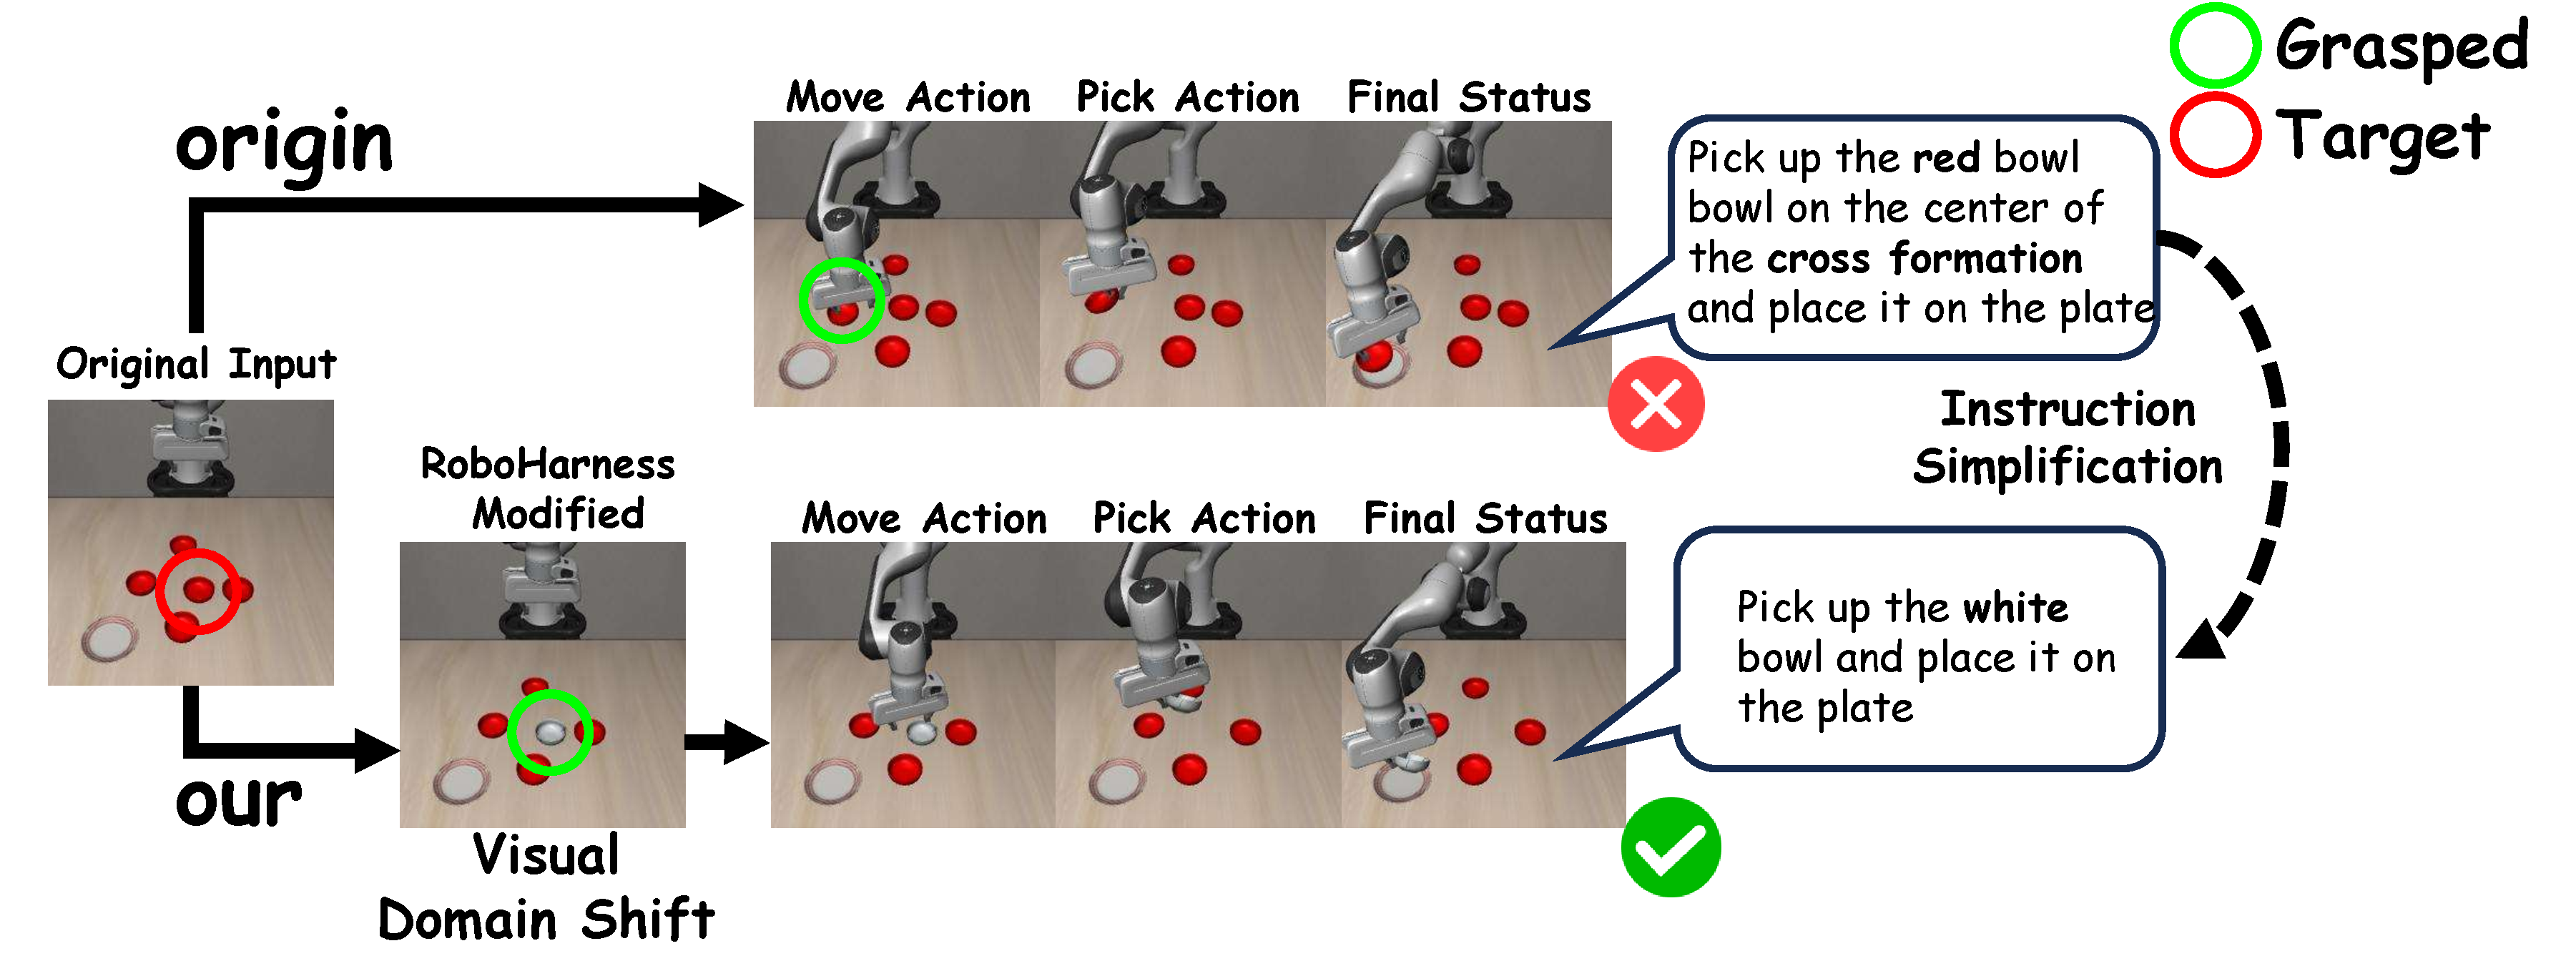
\includegraphics[width=0.95\columnwidth]{figure/visual_shift.pdf}
    \caption{\textbf{视觉聚焦。}处理复杂操作环境中的视觉偏移。}
    \label{fig:visual_shift}
    \vspace{-1em}
\end{figure}
Paint-to-Action 执行非参数域自适应：
\begin{equation}
o_t' = \text{Paint-to-Action}(o_t, \theta_{\text{dist}}).
\end{equation}
它通过 \texttt{visual\_overlay} 和 \texttt{replace\_texture} 实现。
编排器推导 $\theta_{\text{dist}}$，SAM3~\cite{sam3} 分割目标区域，再通过高对比度掩码或成功轨迹中的纹理（\texttt{rag\_success}）缓解偏移（图~\ref{fig:visual_shift}）。

\subsubsection{Eraser：因果混淆}
\begin{figure}[htbp]
    \centering
    \vspace{-0.5em}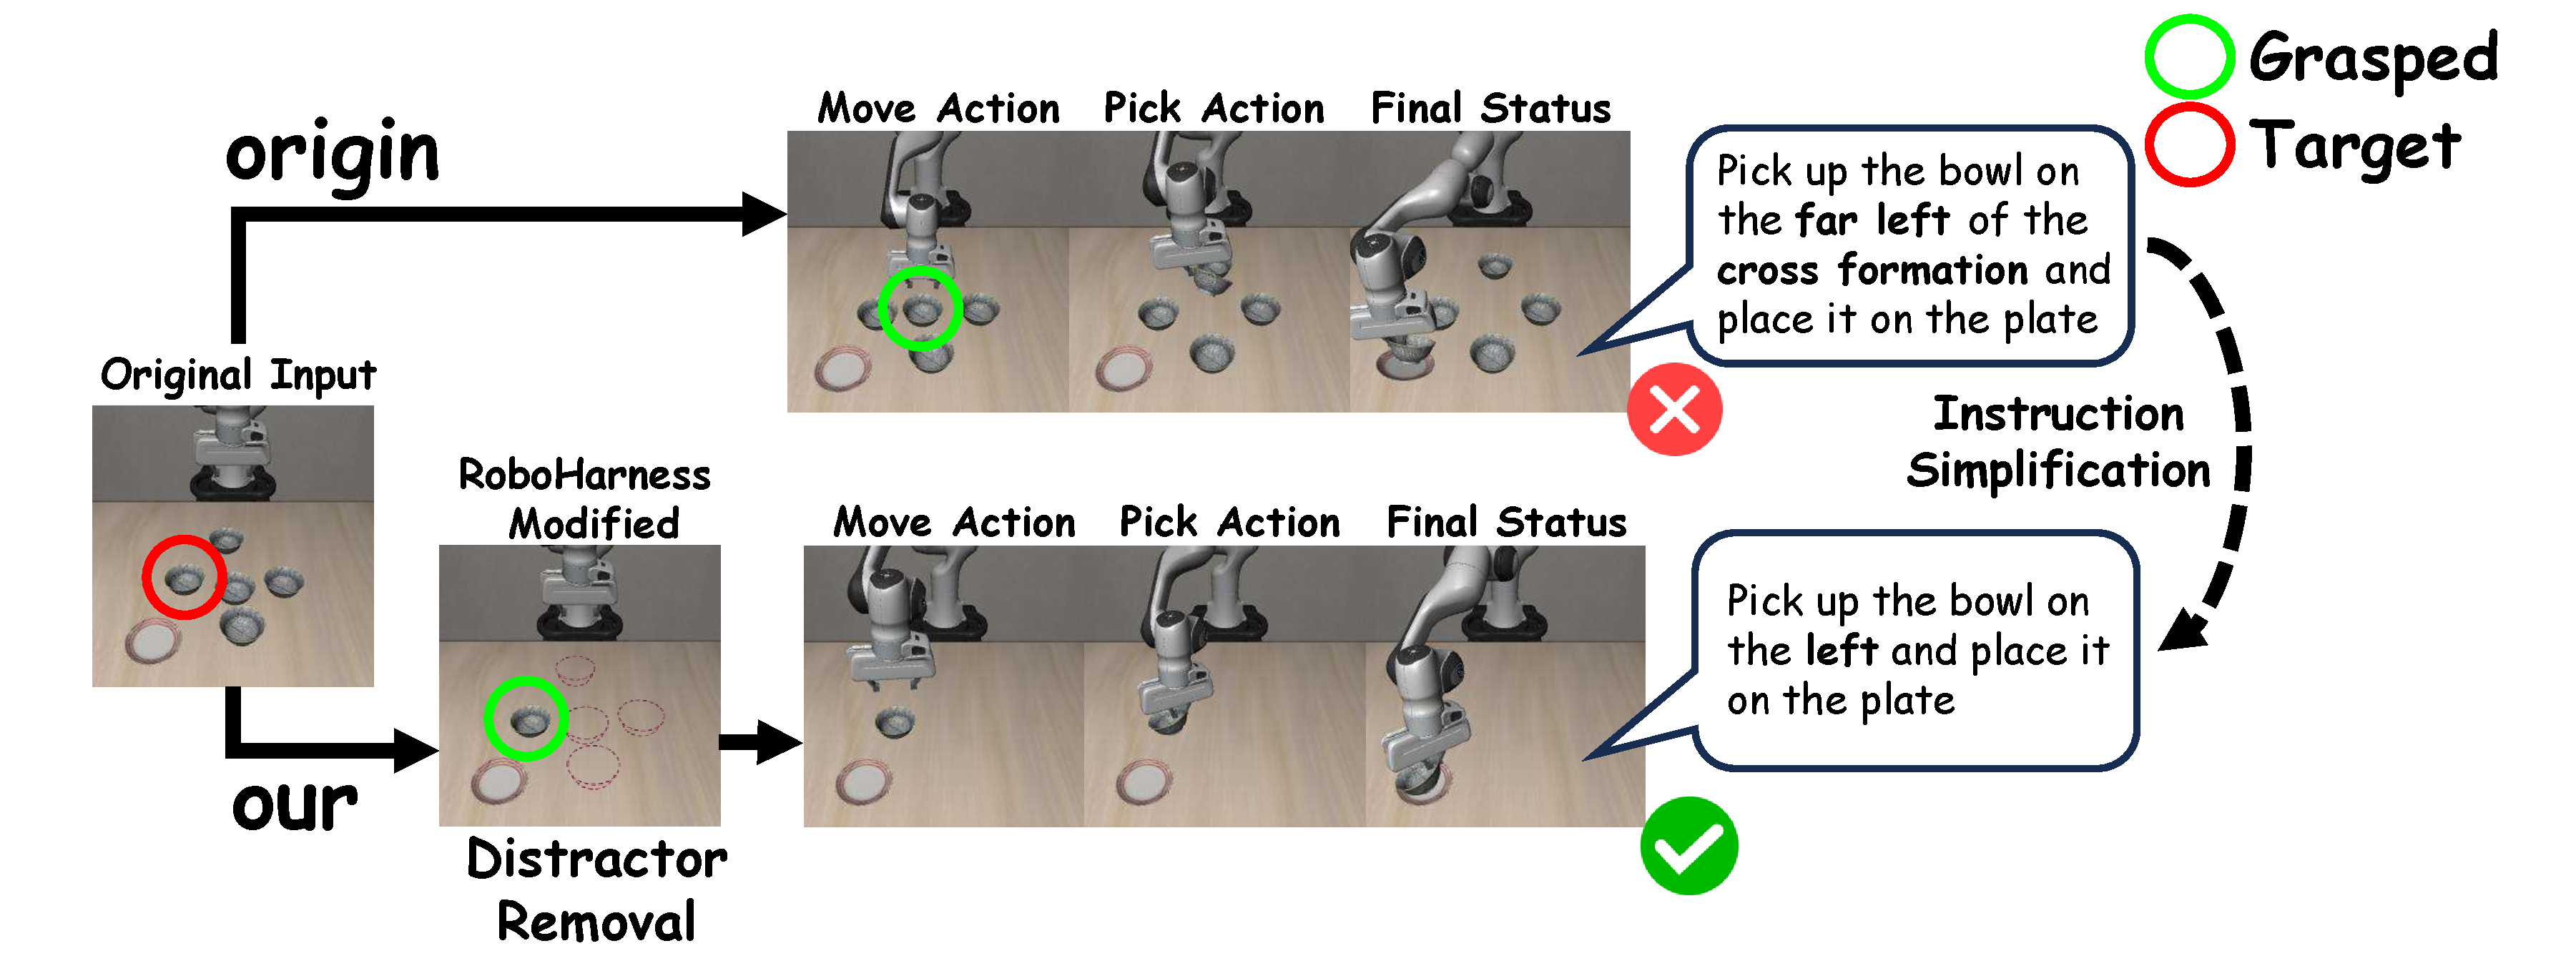
\includegraphics[width=0.95\columnwidth]{figure/remove_distract.pdf}
    \caption{\textbf{杂物移除。}擦除无关干扰物以缓解因果混淆。}
    \label{fig:remove_distract}
    \vspace{-1em}
\end{figure}
Eraser 通过 $\theta_{\text{conf}}$ 移除无关物体：
\begin{equation}
o_t' = \text{Eraser}(o_t, \theta_{\text{conf}}).
\end{equation}
使用 \texttt{remove\_distractor} 时，编排器根据 $o_t$ 和 $\mathcal{H}_t$ 识别干扰物，SAM3~\cite{sam3} 提取掩码，OpenCV Telea 修复算法则在策略推理前移除这些干扰物（图~\ref{fig:remove_distract}）。

\subsubsection{Prompt-Refiner：指令模式不匹配}
\begin{figure}[htbp]
    \centering
    \vspace{-0.5em}
    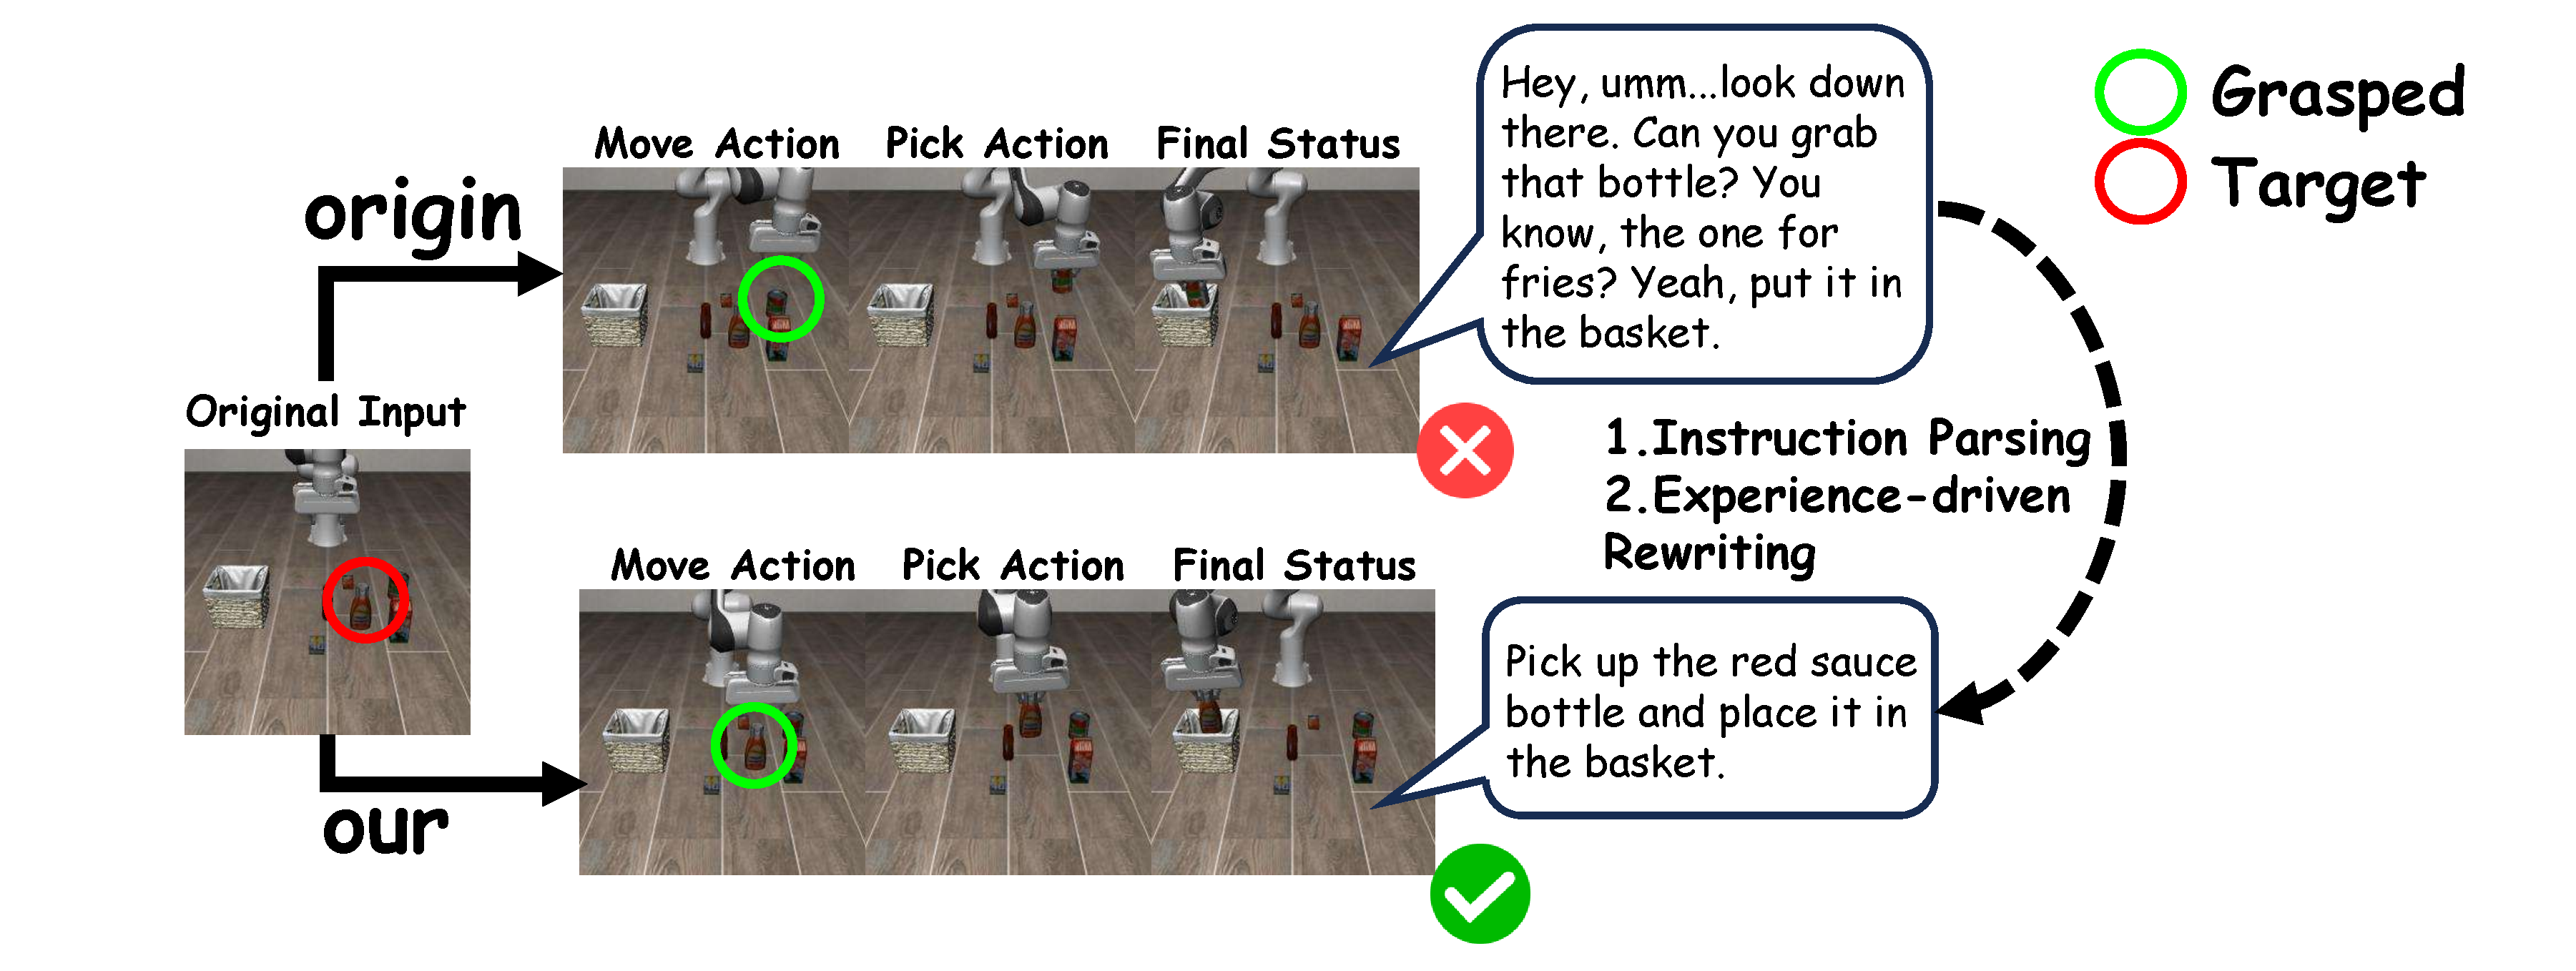
\includegraphics[width=0.95\columnwidth]{figure/prompt_understanding.pdf}
    \caption{\textbf{噪声提示。}将偏离历史成功经验模式的指令改写为简洁、可执行的命令。}
    \label{fig:prompt_understanding}
    \vspace{-1em}
\end{figure}
Prompt-Refiner 改进措辞或任务结构偏离检索成功经验的指令：
\begin{equation}
l_t' = \text{Prompt-Refiner}(l_t, \theta_{\text{lang}}).
\end{equation}
当 $l_t$ 的措辞或任务结构偏离 $\mathcal{H}_t$ 中检索到的成功经验模式时，编排器对其进行改写，生成简洁的 \texttt{refined\_task} 供执行（例如，图~\ref{fig:prompt_understanding} 中的口语化或对话式指令被改写为“Pick\ldots and place\ldots”形式）。

\subsubsection{Chaining-Step：时间复合误差}

Chaining-Step 缩短任务时程：
\begin{equation}
A_{seq}' = \text{Chaining-Step}(A_{seq}, \theta_{\text{chain}}).
\end{equation}
编排器使用 $\mathcal{H}_t$ 将宏观序列 $A_{seq}$ 分解为对齐的子任务，并根据 $\theta_{\text{chain}}$ 指定时间边界（尤其是 $N_e,N_b$）。
以 $A_{seq}'$ 替换 $A_{seq}$ 可缩短执行片段，缓解长时程上下文退化（例如，图~\ref{fig:long_horizon} 中的长任务被拆为更短的子任务，并在其间执行“Reset \& Buffer”）。

\subsubsection{Encore：执行停滞}
\begin{figure}[htbp]
    \vspace{0.5em}
    \centering
    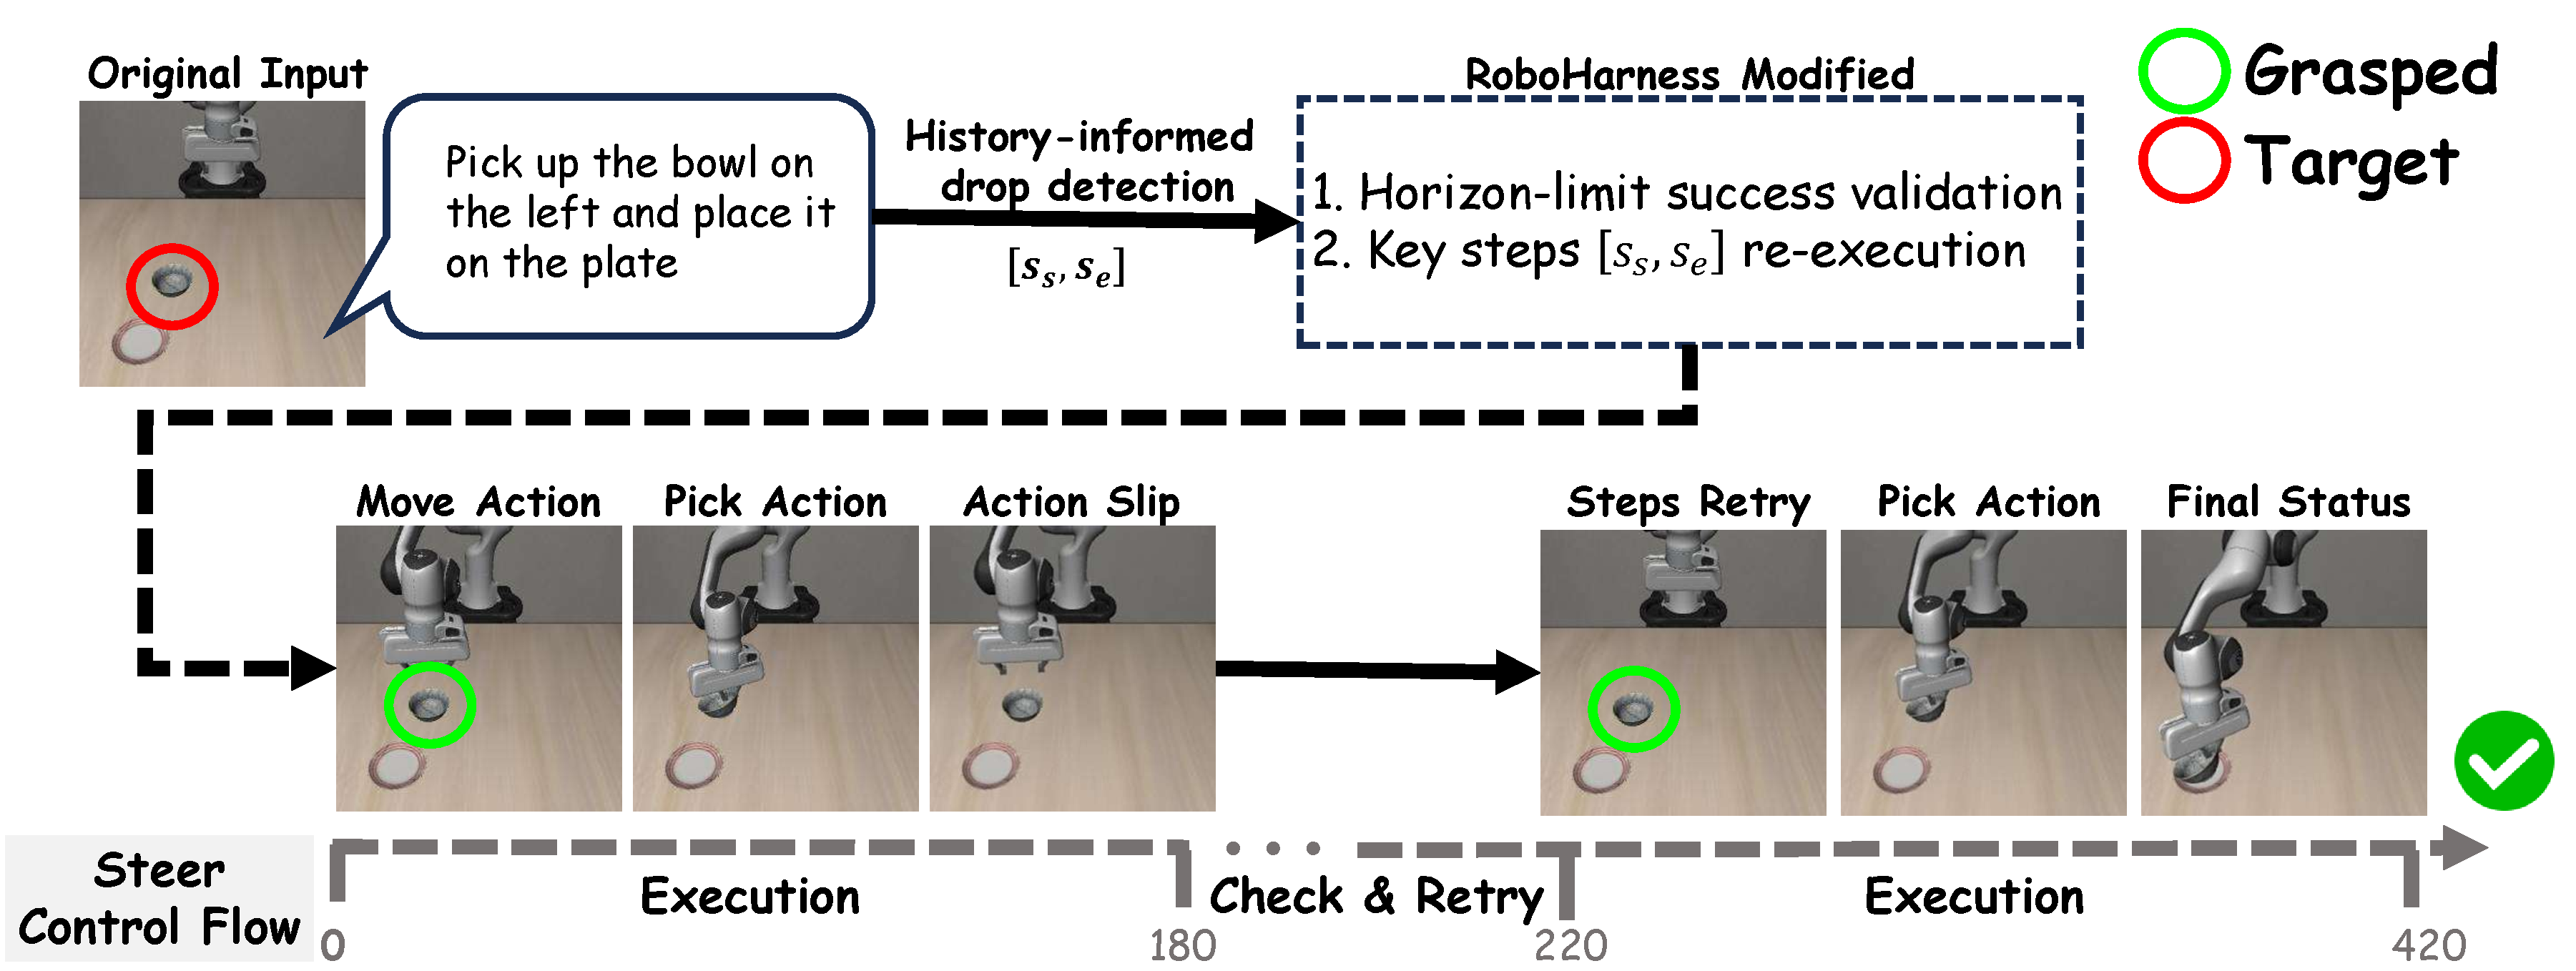
\includegraphics[width=0.95\columnwidth]{figure/encore.pdf}
    \caption{\textbf{Encore。}通过重新执行关键步骤进行恢复。}
    \label{fig:encore}
    \vspace{-1.5em}
\end{figure}
Encore 通过关键状态恢复来解除死锁：
\begin{equation}
s'_t = \text{Encore}(s_t, \theta_{\text{stuc}}).
\end{equation}
其中，$\theta_{\text{stuc}}$（来自 $\mathcal{H}_t$ 中的失败先例）指定重试边界 $[s_s,s_e]$ 和等待时间 $N_w$。
\texttt{encore} 工具重置计数器，并沿平均反向轨迹回滚；若时程上限验证失败，它会从关键帧 $s_s$ 触发“Reset \& Retry”（图~\ref{fig:encore}）。

\subsection{双阶段记忆巩固}
\label{Evolution}

该模块如图~\ref{framework}D 所示，使用双阶段归因机制将最新执行轨迹巩固到双记忆库 $\mathcal{M}$ 中。

\subsubsection{阶段一：初始诊断}

任务终止后，编排器执行初始诊断：
\begin{equation}
e_{new} = \text{InitDiag}(o_t, T_{raw}),
\end{equation}
并存储新经验：
\begin{equation}
\mathcal{M} = \mathcal{M} \cup \{e_{new}\}.
\end{equation}

\subsubsection{阶段二：记忆巩固}

记忆巩固检索最相似的前 $N$ 项经验 $\mathcal{E}_{\text{sim}} = \{e_{\text{sim}}^1, \dots, e_{\text{sim}}^N\}$，以进行跨任务改进：
\begin{equation}
\{e_{\text{new}}^*, e_{\text{sim}}^{1*}, \dots, e_{\text{sim}}^{N*}\} = \text{MemConsol}(e_{\text{new}}, \mathcal{E}_{\text{sim}}),
\end{equation}
其中每个 $e^*$ 都是更新后的经验元组。
编排器进行批次级差分分析，使用新证据纠正历史失败描述并优化修正方案，使 $\mathcal{M}$ 能够迭代自纠正，而非只是单调扩张。

\endinput
